\documentclass[a4paper, 10.5pt, titlepage]{article}
\usepackage{fancyhdr}
\usepackage{graphicx}
\usepackage{imakeidx}
\usepackage{makeidx}
\usepackage{mathtools}
\usepackage[spanish]{babel}
\usepackage{eurosym}

% CODE C
\usepackage{amssymb}
\usepackage{listings}
\usepackage{verbatim}
\usepackage{xcolor}
\definecolor{textblue}{rgb}{.2,.2,.7}
\definecolor{textred}{rgb}{0.54,0,0}
\definecolor{textgreen}{rgb}{0,0.1,0}
\lstset{language=C, 
numbers=left, 
numberstyle=\tiny, 
stepnumber=1,
numbersep=5pt, 
tabsize=4,
basicstyle=\ttfamily,
keywordstyle=\color{textblue},
commentstyle=\color{textred},   
stringstyle=\color{textgreen},
frame=none,                    
columns=fullflexible,
keepspaces=true,
xleftmargin=\parindent,
showstringspaces=false}

\title{LaTeX}
\author{Alberto Fraile}
\date{2020}

\begin{document}

\maketitle
\tableofcontents
\newpage

\section{Elementos y opciones de un documento}

 \begin{verbatim}   


 letterpaper
 a4paper
 a5paper
 b5paper
 legalpaper
 executivepape

 landscape

 10pt
 11pt
 12pt

 oneside
 twoside

 titlepage
 notitlepage

 openright
 openany
 
 onecolumn
 twocolumn
\end{verbatim}   

\newpage

\section{Paquetes comunes}

\newpage

\section{Comandos comunes}

\newpage

\section{La portada del documento}

\newpage

\section{Creación y edición de tablas}

\newpage

\begin{section}{Estructura y desarrollo de un artículo}\end{section}

\begin{lstlisting}
    \documentclass[a4paper, 10pt, titlepage]{article}

    \usepackage{hyperref}
    \usepackage[utf8]{inputenc}
    \usepackage[spanish]{babel}
    \usepackage{graphicx}
    
    \title{Ejemplo}
    \author{Ejempla Ejemplez}
    \date{2020}
    

    \begin{document}

    \maketitle
    \tableofcontents
    
    \\ Nuevo parrafo

    \section{Nombre} 
    \section*{Sin Numeracion}

    \subsection{Nombre} 
    \subsection*{Sin Numeracion}

    \subsubsection{Nombre}

    \textbf{Negrita} \textit{Cursiva} \underline{Subrayado}
    
    \label{'Etiqueta'}
    \ref{'Etiqueta'}

    \begin{quote}
        \small <<Ejemplo de cita>>
    \end{quote}

    \begin{figure}[htp]
        \centering
        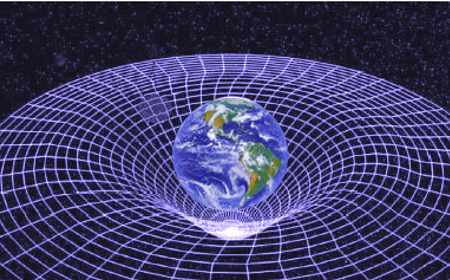
\includegraphics[width=0.8\textwidth]{imagen.jpeg}
        \caption{Descripcion de la fotografia}
        \label{imagenejemplo}
    \end{figure}

    \end{document}
\end{lstlisting}    

\newpage

\begin{section}{Estructura y desarrollo de un libro}\end{section}
   
    \begin{lstlisting}
        \documentclass[a4paper, 10pt, titlepage]{book}
    
        \usepackage{hyperref}
        \usepackage[utf8]{inputenc}
        \usepackage[spanish]{babel}
        \usepackage{graphicx}
        
        \title{Ejemplo}
        \author{Ejempla Ejemplez}
        \date{2020}
        
    
        \begin{document}
    
        \maketitle
        \tableofcontents
        
        \\ Nuevo parrafo
    
        \chapter{Nombre} 
        \chapter*{Sin Numeracion}
    
        \section{Nombre} 
        \section*{Sin Numeracion}
    
        \label{'Etiqueta'}
        \ref{'Etiqueta'}
    
        \begin{quote}
            \small <<Ejemplo de cita>>
        \end{quote}

        \begin{figure}[htp]
            \centering
            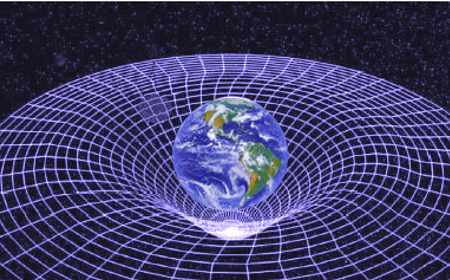
\includegraphics[width=0.8\textwidth]{imagen.jpeg}
            \caption{Descripcion de la fotografia}
            \label{imagenejemplo}
        \end{figure}

        \end{document}\end{lstlisting}      
        
        \small<<Numeración a los costados. Los capítulos comienzan siempre en página impar.>>

\newpage

\section{Estructura y desarrollo de un reporte}

\begin{lstlisting}
    \documentclass[a4paper, 10pt, titlepage]{report}

    \usepackage{hyperref}
    \usepackage[utf8]{inputenc}
    \usepackage[spanish]{babel}
    \usepackage{graphicx}
    
    \title{Ejemplo}
    \author{Ejempla Ejemplez}
    \date{2020}
    

    \begin{document}

    \maketitle
    \tableofcontents
    
    \\ Nuevo parrafo

    \chapter{Nombre} 
    \chapter*{Sin Numeracion}

    \section{Nombre} 
    \section*{Sin Numeracion}

    \label{'Etiqueta'}
    \ref{'Etiqueta'}

    \begin{quote}
        \small <<Ejemplo de cita>>
    \end{quote}

    \begin{figure}[htp]
        \centering
        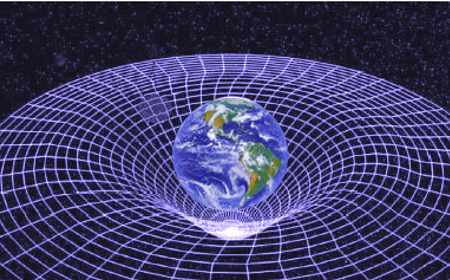
\includegraphics[width=0.8\textwidth]{imagen.jpeg}
        \caption{Descripcion de la fotografia}
        \label{imagenejemplo}
    \end{figure}

    \end{document}\end{lstlisting}      
    
    \small<<Los capítulos comienzan en página siguiente a la finalización del anterior .>>

\newpage 

\section{Estructura y desarrollo de una carta}

\begin{lstlisting}

    \documentclass{letter}
    \usepackage{hyperref}
    \signature{Jorge Carrion}
    \address{21 Menendez Pelayo \\ Sevilla \\ 41000 Sevilla}
    \begin{document}
    
    \begin{letter}{Director \\ Doe \& Co \\ 35 Anthony Road
    \\ Newport \\ Ipswich IP3 5RT}
    \opening{Dear Sir or Madam:}
    
    I am writing to you on behalf of the Wikipedia project (http://www.wikipedia.org/),
    an endeavour to build a fully-fledged multilingual encyclopaedia in an entirely
    open manner, to ask for permission to use your copyrighted material.
    
    % The \ldots command produces dots in a way that will not upset
    % the typesetting of the document.
    \ldots 
    
    That said, allow me to reiterate that your material will be used to the noble end of
    providing a free collection of knowledge for everyone; naturally enough, only if you
    agree. If that is the case, could you kindly fill in the attached form and post it
    back to me? We shall greatly appreciate it.
    
    Thank you for your time and consideration.
    
    I look forward to your reply.
    
    \closing{Yours Faithfully,}
    
    \ps
    
    P.S. You can find the full text of GFDL license at
    \url{http://www.gnu.org/copyleft/fdl.html}.
    
    \encl{Copyright permission form}
    
    \end{letter}
    \end{document}    

\end{lstlisting}


\end{document}